% Options for packages loaded elsewhere
\PassOptionsToPackage{unicode}{hyperref}
\PassOptionsToPackage{hyphens}{url}
\documentclass[
  ignorenonframetext,
]{beamer}
\newif\ifbibliography
\usepackage{pgfpages}
\setbeamertemplate{caption}[numbered]
\setbeamertemplate{caption label separator}{: }
\setbeamercolor{caption name}{fg=normal text.fg}
\beamertemplatenavigationsymbolsempty
% remove section numbering
\setbeamertemplate{part page}{
  \centering
  \begin{beamercolorbox}[sep=16pt,center]{part title}
    \usebeamerfont{part title}\insertpart\par
  \end{beamercolorbox}
}
\setbeamertemplate{section page}{
  \centering
  \begin{beamercolorbox}[sep=12pt,center]{section title}
    \usebeamerfont{section title}\insertsection\par
  \end{beamercolorbox}
}
\setbeamertemplate{subsection page}{
  \centering
  \begin{beamercolorbox}[sep=8pt,center]{subsection title}
    \usebeamerfont{subsection title}\insertsubsection\par
  \end{beamercolorbox}
}
% Prevent slide breaks in the middle of a paragraph
\widowpenalties 1 10000
\raggedbottom
\AtBeginPart{
  \frame{\partpage}
}
\AtBeginSection{
  \ifbibliography
  \else
    \frame{\sectionpage}
  \fi
}
\AtBeginSubsection{
  \frame{\subsectionpage}
}
\usepackage{iftex}
\ifPDFTeX
  \usepackage[T1]{fontenc}
  \usepackage[utf8]{inputenc}
  \usepackage{textcomp} % provide euro and other symbols
\else % if luatex or xetex
  \usepackage{unicode-math} % this also loads fontspec
  \defaultfontfeatures{Scale=MatchLowercase}
  \defaultfontfeatures[\rmfamily]{Ligatures=TeX,Scale=1}
\fi
\usepackage{lmodern}
\ifPDFTeX\else
  % xetex/luatex font selection
\fi
% Use upquote if available, for straight quotes in verbatim environments
\IfFileExists{upquote.sty}{\usepackage{upquote}}{}
\IfFileExists{microtype.sty}{% use microtype if available
  \usepackage[]{microtype}
  \UseMicrotypeSet[protrusion]{basicmath} % disable protrusion for tt fonts
}{}
\makeatletter
\@ifundefined{KOMAClassName}{% if non-KOMA class
  \IfFileExists{parskip.sty}{%
    \usepackage{parskip}
  }{% else
    \setlength{\parindent}{0pt}
    \setlength{\parskip}{6pt plus 2pt minus 1pt}}
}{% if KOMA class
  \KOMAoptions{parskip=half}}
\makeatother
\usepackage{graphicx}
\makeatletter
\newsavebox\pandoc@box
\newcommand*\pandocbounded[1]{% scales image to fit in text height/width
  \sbox\pandoc@box{#1}%
  \Gscale@div\@tempa{\textheight}{\dimexpr\ht\pandoc@box+\dp\pandoc@box\relax}%
  \Gscale@div\@tempb{\linewidth}{\wd\pandoc@box}%
  \ifdim\@tempb\p@<\@tempa\p@\let\@tempa\@tempb\fi% select the smaller of both
  \ifdim\@tempa\p@<\p@\scalebox{\@tempa}{\usebox\pandoc@box}%
  \else\usebox{\pandoc@box}%
  \fi%
}
% Set default figure placement to htbp
\def\fps@figure{htbp}
\makeatother
\setlength{\emergencystretch}{3em} % prevent overfull lines
\providecommand{\tightlist}{%
  \setlength{\itemsep}{0pt}\setlength{\parskip}{0pt}}
\usepackage{bookmark}
\IfFileExists{xurl.sty}{\usepackage{xurl}}{} % add URL line breaks if available
\urlstyle{same}
\hypersetup{
  hidelinks,
  pdfcreator={LaTeX via pandoc}}

\author{\texorpdfstring{}{}}
\date{}

\begin{document}

\begin{frame}[fragile]{Methods: Synthesis, gaps, and coverage scores}
\protect\phantomsection\label{methods-synthesis-gaps-and-coverage-scores}
\textbf{Synthesis} (\texttt{src/synthesis.py}) maps each handbook
section to the tuple of evidence items whose themes intersect the
section's \texttt{theme\_ids}. The \textbf{coverage score} is computed
by \texttt{section\_coverage\_score()}: the sum of weights for that
section, capped at \(1.0\), so many weak items cannot masquerade as
certainty.

Sections whose score is \textbf{strictly below} the configured gap
threshold (default \texttt{DEFAULT\_GAP\_THRESHOLD\ =\ 0.35}) are listed
in \texttt{gaps}. Callers may pass
\texttt{synthesize(corpus,\ gap\_threshold=…)} when a stricter or looser
policy applies; the chosen value is stored on
\texttt{SynthesisResult.gap\_threshold} and echoed in JSON metrics via
\texttt{build\_metrics\_report()} (\texttt{gap\_threshold},
\texttt{gap\_section\_ids}, \texttt{gap\_count}).

Figure \ref{fig:coverage} shows section-level scores for the Riverbend
fixture. Figure \ref{fig:bytheme} shows how many evidence rows attach to
each theme id in the same fixture. Figure \ref{fig:gapstatus} repeats
the section ordering used in metrics export (sorted ids) and colors bars
by membership in \texttt{gap\_section\_ids}, so readers can see which
chapters would be flagged without rereading JSON.

\begin{figure}
\centering
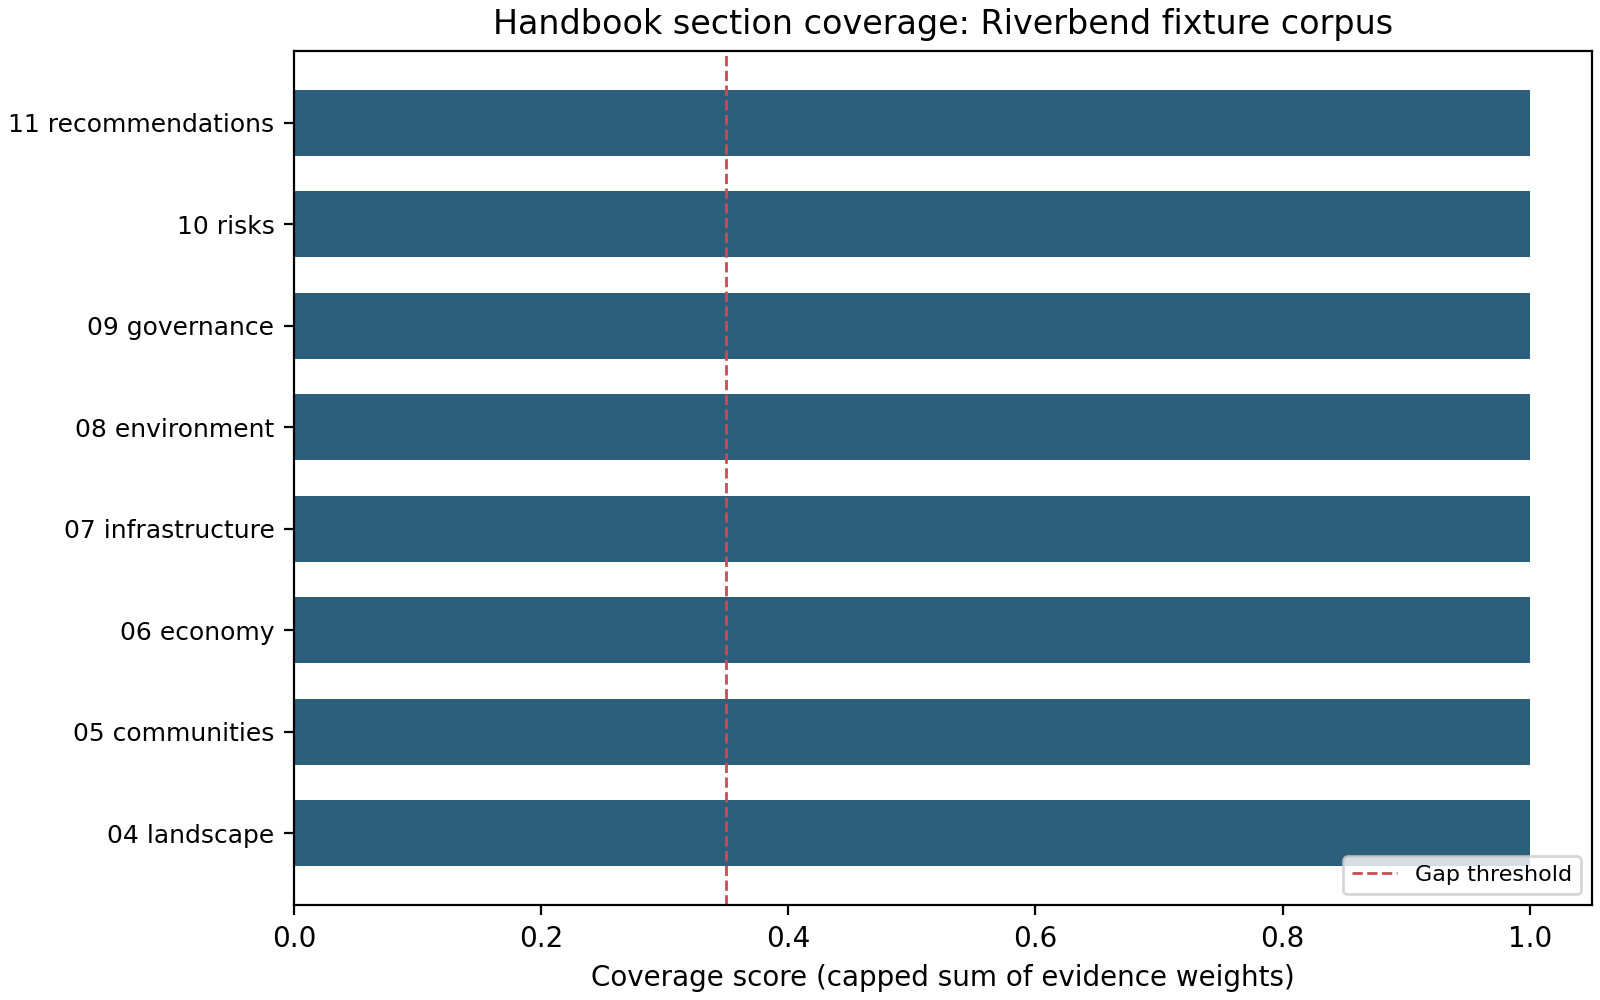
\includegraphics[width=0.85\linewidth,height=\textheight,keepaspectratio,alt={Riverbend fixture (version 2026.1): horizontal coverage score per handbook section (capped sum of matching evidence weights, range 0--1). Red dashed vertical line: current gap threshold from synthesis; sections strictly to the left would be listed in the JSON gaps array.}]{../figures/handbook_evidence_coverage.png}
\caption{Riverbend fixture (version 2026.1): horizontal coverage score
per handbook section (capped sum of matching evidence weights, range
0--1). Red dashed vertical line: current gap threshold from synthesis;
sections strictly to the left would be listed in the JSON gaps
array.}\label{fig:coverage}
\end{figure}

Under the default threshold, the Riverbend exemplar places every outline
section at or above the line (\texttt{gap\_count} is zero in
\texttt{handbook\_report.json}), which is why the executive summary can
describe a ``fully covered'' template run. The chart still documents the
contract: any future corpus revision that drags a section left of the
dashed line will surface automatically in the gap table from
\texttt{build\_gap\_report\_md()} and in pipeline metrics.

\begin{figure}
\centering
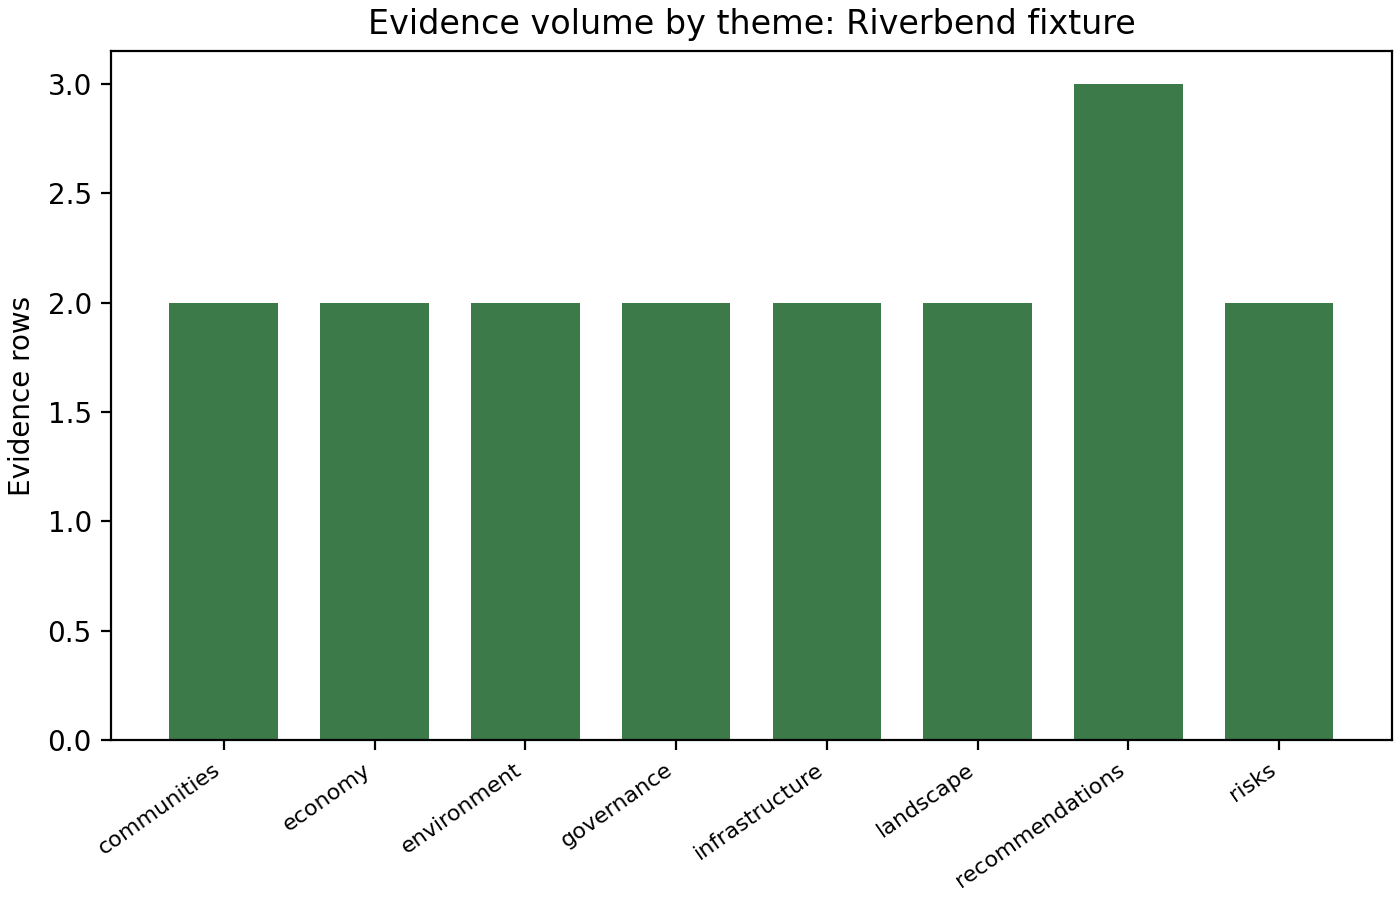
\includegraphics[width=0.8\linewidth,height=\textheight,keepaspectratio,alt={Riverbend fixture: count of evidence rows per theme id after corpus validation (duplicate ids and invalid weights rejected at load). Bar height shows how many statements contribute to each thematic bucket used for section routing.}]{../figures/handbook_evidence_by_theme.png}
\caption{Riverbend fixture: count of evidence rows per theme id after
corpus validation (duplicate ids and invalid weights rejected at load).
Bar height shows how many statements contribute to each thematic bucket
used for section routing.}\label{fig:bytheme}
\end{figure}

The histogram is intentionally simple: it answers whether evidence
volume is balanced across themes or concentrated in a few buckets. For
Riverbend, economy, infrastructure, and recommendations each carry
multiple rows, while every declared theme has at least one row
(\texttt{themes\_without\_evidence} is empty). Editors use this view to
spot missing thematic coverage before rewriting chapter prose.

\begin{figure}
\centering
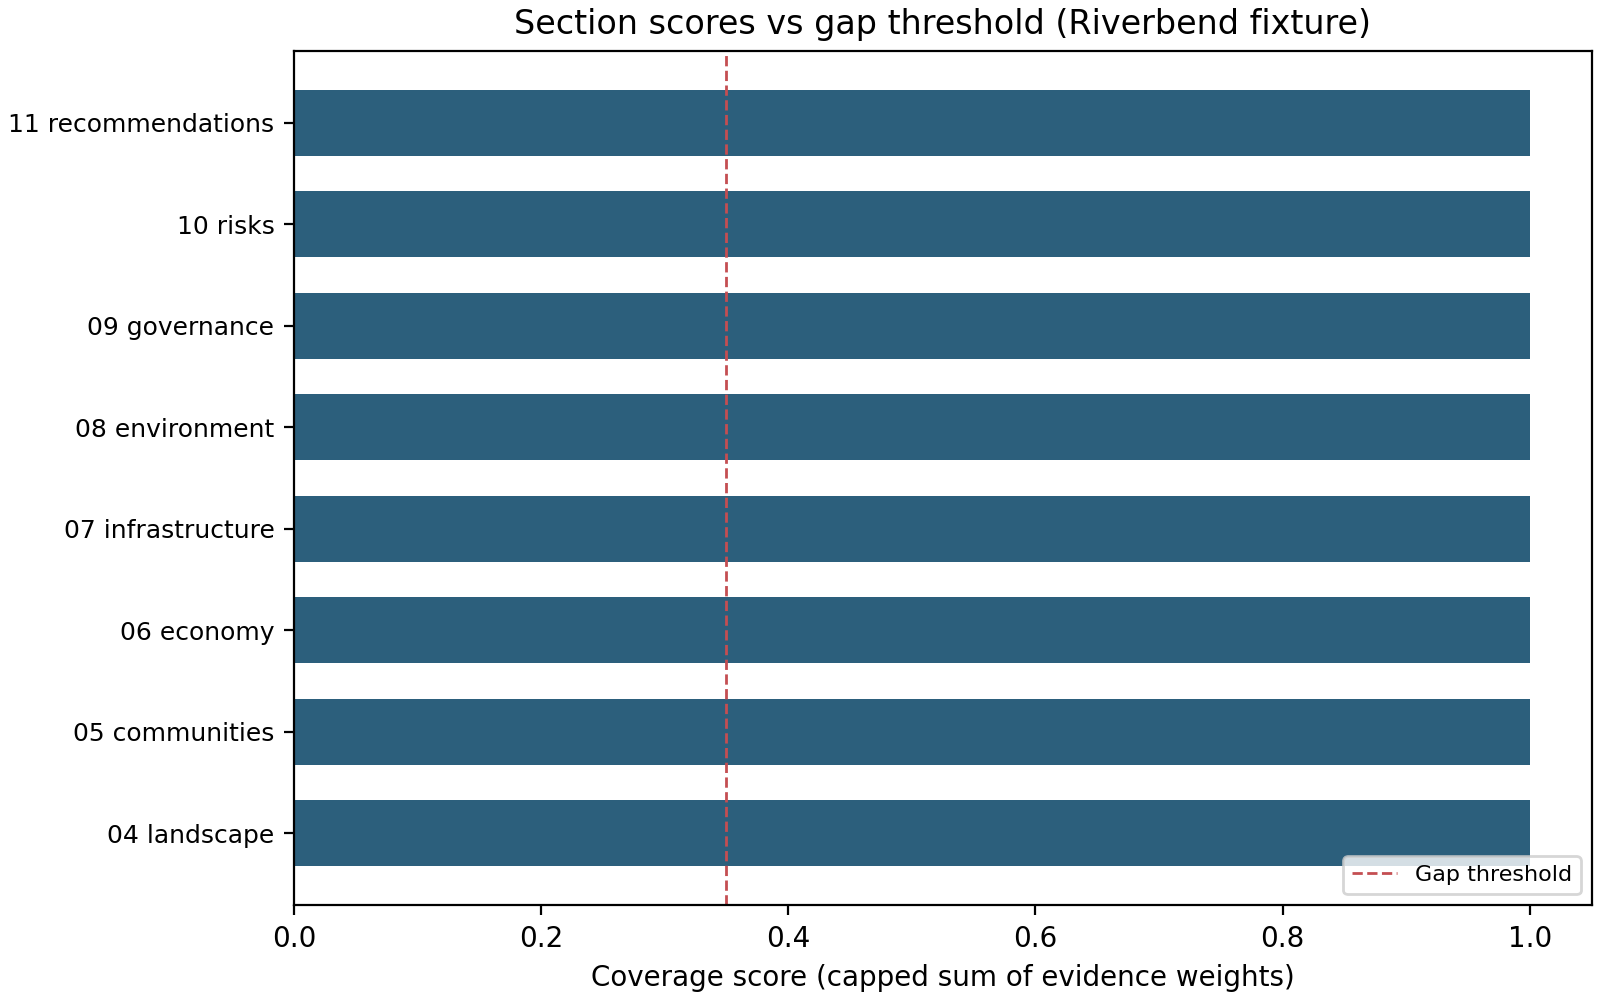
\includegraphics[width=0.85\linewidth,height=\textheight,keepaspectratio,alt={Same scores as the coverage chart, sorted by section id, with bars colored by gap status: coral = section id in gap\_section\_ids (score strictly below threshold); steel blue = at or above threshold. For this fixture under the default threshold, all sections are above the line (empty gap list), illustrating a fully covered outline.}]{../figures/handbook_section_gap_status.png}
\caption{Same scores as the coverage chart, sorted by section id, with
bars colored by gap status: coral = section id in gap\_section\_ids
(score strictly below threshold); steel blue = at or above threshold.
For this fixture under the default threshold, all sections are above the
line (empty gap list), illustrating a fully covered
outline.}\label{fig:gapstatus}
\end{figure}

When \texttt{gap\_section\_ids} is non-empty, coral bars identify
exactly which sections require new evidence or threshold tuning before
publication. The sort order matches \texttt{scores\_by\_section} keys in
JSON, which keeps figure inspection aligned with diff review of
\texttt{handbook\_report.json}.

Markdown bodies for preview or annex publication are assembled in
\texttt{src/handbook\_md.py}: executive bullets, gap table,
evidence-by-theme table, per-section evidence lists, and optional
\texttt{build\_toc\_md()} for outline-only exports.
\end{frame}

\end{document}
